\section{Mindmap Drawing Library}

\begin{package}{pgflibrarytikzmindmap}
  This packages provides styles for drawing mindmap diagrams.
\end{package}

\subsection{Overview}

This library is intended to make the creation of mindmaps easier. A
\emph{mindmap} is a graphical representation of a concept together
with related concepts and annotations. Mindmaps are, essentially,
trees, possibly with a few extra edges added, but they are usually
drawn in a special way: The root concept is placed in the middle of
the page and is drawn as a huge circle, ellipse, or cloud. The related
concepts then ``leave'' this root concept in branch-like tendrils.

The mindmap library of \tikzname\ produces mindmaps that look a bit
different from the standard mindmaps: While the big root concept is
still a circle, related concepts are also depicted as (smaller)
circles. The related concepts are linked to the root concept via
organic-looking connections. The overall effect is visually rather
pleasing, but readers may not immediately think of a mindmap when they
see a picture created with this library.

Although it is not strictly necessary, you will usually create
mindmaps using \tikzname's tree mechanism and some of the styles and
macros of the package work best when used inside trees. However, it is
still possible and sometimes necessary to treat parts of a mindmap as
a graph with arbitrary edges and this is also possible.


\subsection{The Mindmap Style}

Every mindmap should be put in a scope or a picture where the
|mindmap| style is used. This style installs some internal settings.

\begin{itemize}
  \itemstyle{mindmap}
  Use this style with all pictures or at least scopes that contain a
  mindmap. It installs a whole bunch of settings that are useful for
  drawing mindmaps. 
\begin{codeexample}[]
\tikz[mindmap,concept color=red!50]
  \node [concept] {Root concept}
    child[grow=right] {node[concept] {Child concept}};
\end{codeexample}
  The sizes of concepts are predefined in such a way that a
  medium-size mindmap will fit on an A4 page (more or less).  
  \itemstyle{every mindmap}
  This style is included by the |mindmap| style. Change this style to
  add special settings to your mindmaps.
\begin{codeexample}[]
\tikz[large mindmap,concept color=red!50]
  \node [concept] {Root concept}
    child[grow=right] {node[concept] {Child concept}};
\end{codeexample}
  \itemstyle{large mindmap}
  This style includes the |mindmap| style, but additionally changes
  the default size of concepts and of distances so that a medium-sized
  mindmap will fit on an A3 page (A3 pages are twice as large as A4
  pages).
  \itemstyle{huge mindmap}
  This style causes conepts to be even bigger and it is best used with
  A2 paper and above.
\end{itemize}

\subsection{Concepts Nodes}

The basic entities of mindmaps are called \emph{concepts} in
\tikzname. A concept is a node of style |concept| and it must be
circular for some of the connection macros to work.


\subsubsection{Isolated Concepts}

The following styles influence how isolated concepts are rendered:

\begin{itemize}
  \itemstyle{concept}
  This style should be used with all nodes that are concepts, although
  some styles like |extra concept| install this style automatically.

  Bascially, this style makes the concept node circular and installs a
  uniform color called |concept color|, see below. Additionally, the
  style |every concept| is called.
\begin{codeexample}[]
\tikz[mindmap,concept color=red!50] \node [concept] {Some concept};
\end{codeexample}
  \itemstyle{every concept}
  In order to change the appearance of concept nodes, you should
  change this style. Note, however, that the color of a concept should
  be uniform for some of the connection bar stuff to work, so you
  should not change the color or the draw/fill state of concepts using
  this option. It is mostly useful for changing the text color and
  font.
  \itemoption{concept color}|=|\meta{color}
  This option tells \tikzname\ which color should be used for filling
  and stroking concepts. The difference between this option and just
  setting |every concept| to the desired color is that this option
  allows \tikzname\ to keep track of the colors used for
  concepts. This is important when you \emph{change} the color between
  two connected concepts. In this case, \tikzname\ can automatically
  create a shading that provides a smooth transition between the old
  and the new concept color; we will come back to this in the next
  section. 
  \itemstyle{extra concept}
  This style is intended for concepts that are not part of the
  ``mindmap tree,'' but stand beside it. Typically, they will have a
  subdued color are be smaller. In order to have these concepts appear
  in a uniform way and in order to indicate in the code that these
  concepts are extra, you can use this style.
\begin{codeexample}[]
\begin{tikzpicture}[mindmap,concept color=blue!80]
  \node [concept]                 {Root concept};
  \node [extra concept] at (10,0) {extra concept};
\end{tikzpicture}
\end{codeexample}
  \itemstyle{every extra concept}
  Change this style to change the appearance of extra concepts.
\end{itemize}


\subsubsection{Concepts in Trees}

As pointed out earlier, \tikzname\ assumes that your mindmap is build
using the |child| facilities of \tikzname. There are numerous options
that influence how concepts are rendered at the different levels of a
tree. 

\begin{itemize}
  \itemstyle{root concept}
  This style is used for the roots of mindmap trees. More precisely,
  this style is included by the |mindmap| style. Thus, by adding
  something to this, you can change how the root of a mindmap will be
  rendered.
\begin{codeexample}[]
\tikzstyle{root concept}+=[concept color=blue!80,minimum size=3.5cm]    
\tikz[mindmap] \node [concept] {Root concept};
\end{codeexample}

  Note that styles like |large mindmap| redefine these styles, so you
  should add something to this style only inside the picture.
  \itemstyle{level 1 concept}
  The |mindmap| style adds this style to the |level 1| style. This
  means that the first level children of a mindmap tree will use this
  style. 
\begin{codeexample}[]
\tikzstyle{root concept}+=[concept color=blue!80]    
\tikzstyle{level 1 concept}+=[concept color=red!50]    
\tikz[mindmap]
  \node [concept] {Root concept}
    child[grow=30] {node[concept] {child}}
    child[grow=0 ] {node[concept] {child}};
\end{codeexample}
  \itemstyle{level 2 concept}
  works like |level 1 concept|, only for second level children. 
  \itemstyle{level 3 concept}
  works like |level 1 concept|.
  \itemstyle{level 4 concept}
  works like |level 1 concept|. Note that there are not fifth and
  higher level styles, you need to modify |level 5| directly in such
  cases. 
  
  \itemoption{concept color}|=|\meta{color}
  We saw already that this option is used to change the color of
  concepts. We now have a look at its effect when used on child nodes
  of a concept. Normally, this option simply changes the color of the
  children. However, when the option is given as an option to the
  |child| operation (and not to the |node| operation and also not as
  an option to all children via the |level 1| style), \tikzname\ will
  smoothly change the concept color from the parent's color to the
  color of the child concept. 

  Here is an example:
\begin{codeexample}[]
\tikz[mindmap,concept color=blue!80]
  \node [concept] {Root concept}
    child[concept color=red,grow=30] {node[concept] {Child concept}}
    child[concept color=orange,grow=0]  {node[concept] {Child concept}};
\end{codeexample}

  In order to have all children of a certain level have a different
  concept color, a tiny bit of magic is needed:
\begin{codeexample}[]
\tikzstyle{root concept}+=[concept color=blue]    
\tikzstyle{level 1 concept}+=[set style={{every child}=[concept color=blue!50]}]    
\tikz[mindmap,text=white]
  \node [concept] {Root concept}
    child[grow=30] {node[concept] {child}}
    child[grow=0 ] {node[concept] {child}};
\end{codeexample}
\end{itemize}

\subsection{Connecting Concepts}

\subsubsection{Simple Connections}

The easiest way to connect two concepts is to draw a line between
them. In order to give such lines a consistent appearance, it is
recommendable to use the following style when drawing such lines:

\begin{itemize}
  \itemstyle{concept connection}
  This style can be used for lines between two concepts. Feel free to
  redefine this style.
\end{itemize}

A problem arises when you need to connect concepts after the main
mindmap has been drawn. In this case you will want the connection
lines to lie \emph{behind} the main mindmap. However, you can draw the
lines only after the coordinates of the concepts have been
determined. In this case you should place the connecting lines on a
background layer as in the following example:

\begin{codeexample}[]
\tikzstyle{root concept}+=[concept color=blue!20,minimum size=2cm]    
\tikzstyle{level 1 concept}+=[sibling angle=45]
\begin{tikzpicture}[mindmap]
  \node [concept] {Root concept}
    [clockwise from=45]
    child { node[concept] (c1) {child}}
    child { node[concept] (c2) {child}}
    child { node[concept] (c3) {child}};
  \begin{pgfonlayer}{background}
    \draw [concept connection]  (c1) edge (c2)
                                     edge (c3)
                                (c2) edge (c3);
  \end{pgfonlayer}
\end{tikzpicture}
\end{codeexample}


\subsubsection{The Circle Connection Bar Snake}

Instead of a simple line between two concepts, you can also add a bar
between the two nodes that has slightly organic ends. These bars are
also used by default as the edges from parents in the mindmap tree.

For the drawing of the bars a special snake is used, which is defined
in the mindmap library:

\begin{snake}{circle connection bar}
  This snake can be used to connect two circles. The start of the
  snake should lie on the border of the first circle, the end should
  lie on the border of the second circle. The following two macros should be
  initialized with the sizes of the circles:
  \begin{itemize}
  \item |\pgfsnakecirclestartradius|
  \item |\pgfsnakecircleendradius|
  \end{itemize}
  Furthermore, the following two macros influence the snake:
  \begin{itemize}
  \item |\pgfsnakesegmentamplitude|
  \item |\pgfsnakesegmentangle|
  \end{itemize}
  The snake itself will be a path that starts on the border of the
  first circle at the specified angle relative to the line connecting
  the centers of the circles. The path then changes into a rectangle
  whose thickness is given by the amplitude. Finally, the path ends
  with the same angles on the second circle. 

  Here is an example that should make this clearer:
\begin{codeexample}[]
\begin{tikzpicture}
  \fill[blue!20] (0,0) circle   (1cm);
  \fill[red!20]  (2.5,0) circle (.5cm);

  \def\pgfsnakecirclestartradius{1cm}
  \def\pgfsnakecircleendradius{.5cm}
  \def\pgfsnakesegmentamplitude{2mm}
  \def\pgfsnakesegmentangle{30}

  \filldraw [draw=red,fill=black,snake=circle connection bar] (1,0) -- (2,0);
\end{tikzpicture}
\end{codeexample}

  As can be seen, the snake consists of three parts and is not really
  useful for drawing. However, if you fill the snake only and if you
  use the same color as for the circles, the result is better.
\begin{codeexample}[]
\begin{tikzpicture}[blue!50]
  \fill (0,0) circle   (1cm);
  \fill  (2.5,0) circle (.5cm);

  \def\pgfsnakecirclestartradius{1cm}
  \def\pgfsnakecircleendradius{.5cm}
  \def\pgfsnakesegmentamplitude{2mm}
  \def\pgfsnakesegmentangle{30}

  \fill [snake=circle connection bar] (1,0) -- (2,0);
\end{tikzpicture}
\end{codeexample}

  In the above example you may notice the small white line between the
  circles and the snake. This is due to rounding
  errors. Unfortunately, for larger distances, there errors can
  accumulate quite strongly, especially since \tikzname\ and \TeX\ are
  not very good at computing square roots. For this reason, it is a
  good idea to make the circles slightly larger to cover up such
  problems. When using nodes of shape |circle|, you can just add the
  |draw| option with a |line width| or one or two points (for very
  large distances you may need line width up to 4pt). 
\begin{codeexample}[]
\begin{tikzpicture}[blue!50]
  \fill (0,0) circle   (1cm+1pt);
  \fill  (2.4,0) circle (.5cm+1pt);

  \def\pgfsnakecirclestartradius{1cm}
  \def\pgfsnakecircleendradius{.5cm}
  \def\pgfsnakesegmentamplitude{2mm}
  \def\pgfsnakesegmentangle{30}

  \fill [snake=circle connection bar] (1,0) -- (1.9,0);
\end{tikzpicture}
\end{codeexample}

  Note the slightly strange |outer sep=0pt|. This is needed so that
  the snakes being on the border of the filled circle, not on the
  border of the stroked circle (which is slightly larger and this
  slightly larger size is exactly what we wish to use to cover up the
  rounding errors).
\end{snake}



\subsubsection{The Circle Connection Bar To-Path}

The circle connection bar snake is a bit complicated to
use. Especially specifying the radii is quite bothersome (the
amplitude and the angle can be set once and for all). For this reason,
the mindmap library defines a special to-path, that performs the
necessary computations for you.

\begin{itemize}
  \itemstyle{circle connection bar}
  This style installs a rather involved to-path. Unlike normal
  to-paths, this path requires that the start and the target of the
  to-path are named nodes of shape |circle| -- if this is not the case,
  this path will produce errors.

  Assuming that the start and the target are circles, the to-path will
  first compute the radii of these circles (by measuring the distance
  from the |center| anchor to some anchor on the border) and will set
  the |\pgfsnakecirlce...| macros accordingly. Next, the |fill| option
  is set to the |concept color| while |draw=none| is set. The snake is
  set to |circle conncetion bar|. Finally, the following style is
  included:
  \begin{itemize}
    \itemstyle{every circle connection bar}
    Redefine this sytle to change the appearance of circle connection
    bar to-paths.      
  \end{itemize}
\begin{codeexample}[]
\begin{tikzpicture}[concept color=blue!50,blue!50,outer sep=0pt]
  \node (n1) at (0,0)   [circle,minimum size=2cm,fill,draw,thick] {};
  \node (n2) at (2.5,0) [circle,minimum size=1cm,fill,draw,thick] {};

  \path (n1) to[circle connection bar] (n2);
\end{tikzpicture}
\end{codeexample}
  Note that it is not a good idea to have more than one |to| operation
  together this the option |circle connection bar| in a single
  |\path|. Use the |edge| operation, instead, for creating multiple
  connections and this operation creates a new scope for each edge.
\end{itemize}

In a mindmap we sometimes want colors to change from one concept color
to another. Then, the connection bar should, ideally, consist of a
smooth transition between these two colors. Getting this right using
shadings is a bit tricky if you try this ``by hand,'' so the  mindmap
library provides a special option for facilitating this procedure.

\begin{itemize}
  \itemoption{circle connection bar switch color}|=from (|\meta{first
    color}|) to (|\meta{second color}|)|
  This style works similarly to the |circle connection bar|. The only
  difference is that instead of filling the path with a single color a
  shading is used.
\begin{codeexample}[]
\begin{tikzpicture}[outer sep=0pt]
  \node (n1) at (0,0)    [circle,minimum size=2cm,fill,draw,thick,red] {};
  \node (n2) at (30:2.5) [circle,minimum size=1cm,fill,draw,thick,blue] {};

  \path (n1) to[circle connection bar switch color=from (red) to (blue)] (n2);
\end{tikzpicture}  
\end{codeexample}
\end{itemize}


\subsubsection{Tree Edges}

Most of the time, concepts in a mindmap are connected automatically
when the mindmap is build as a tree. The reason is that the |mindmap|
installs a |circle connection bar| path as the edge from parent
path. Also, the |mindmap| option takes care of things like setting the
correct |draw| and |outer sep| settings and some other stuff.

In detail, the |mindmap| option sets the |edge from parent path| to a
path that uses the to-path |circle connection bar| to connect the parent node
and the child node. The |concept color| option (locally) changes this
by using |circle connection bar switch color| instead with the
from-color set to the old (parent's) concept color and the to-color
set to the new (child's) concept color. This menas that when you
provide the |concept color| option to a |child| command, the color
will change from the parent's concept color to the specified color.

Here is an example of a tree build in this way:

\begin{codeexample}[]
\begin{tikzpicture}
  \path[mindmap,concept color=black,text=white]
    node[concept] {Computer Science}
    [clockwise from=0]
    child[concept color=green!50!black] {
      node[concept] {practical}
      [clockwise from=90]
      child { node[concept] {algorithms} }
      child { node[concept] {data structures} }
      child { node[concept] {pro\-gramming languages} }
      child { node[concept] {software engineer\-ing} }
    }  
    child[concept color=blue] {
      node[concept] {applied}
      [clockwise from=-30]
      child { node[concept] {databases} }
      child { node[concept] {WWW} }
    }
    child[concept color=red] { node[concept] {technical} }
    child[concept color=orange] { node[concept] {theoretical} };
\end{tikzpicture}
\end{codeexample}



\subsection{Adding Annotations}

An \emph{annotation} is some text outside a mindmap that, unlike an
extra concept, simply explains something in the mindmap. The following
style is mainly intended to help readers of the code see that a node
in an annotation node.

\begin{itemize}
  \itemstyle{annotation}
  This style indicates that a node is an annotation node. It includes
  the style |every annotation|, which allows you to change this style
  in a convenient fashion.
\begin{codeexample}[]
\tikzstyle{every annotation}=[fill=red!20]    
\begin{tikzpicture}[mindmap,concept color=blue!80]
  \node [concept] (root)  {Root concept};

  \node [annotation,right] at (root.east)
  {The root concept is, in general, the most important concept.};
\end{tikzpicture}
\end{codeexample}
  \itemstyle{every annotation}
    This style is included by |annotation|.
\end{itemize}


\subsection{Examples}

The following pictures show examples of more complicated mindmaps that
have been created using the mindmap library. Note that these mindmaps
should be printed on A1 paper.

\medskip
\noindent
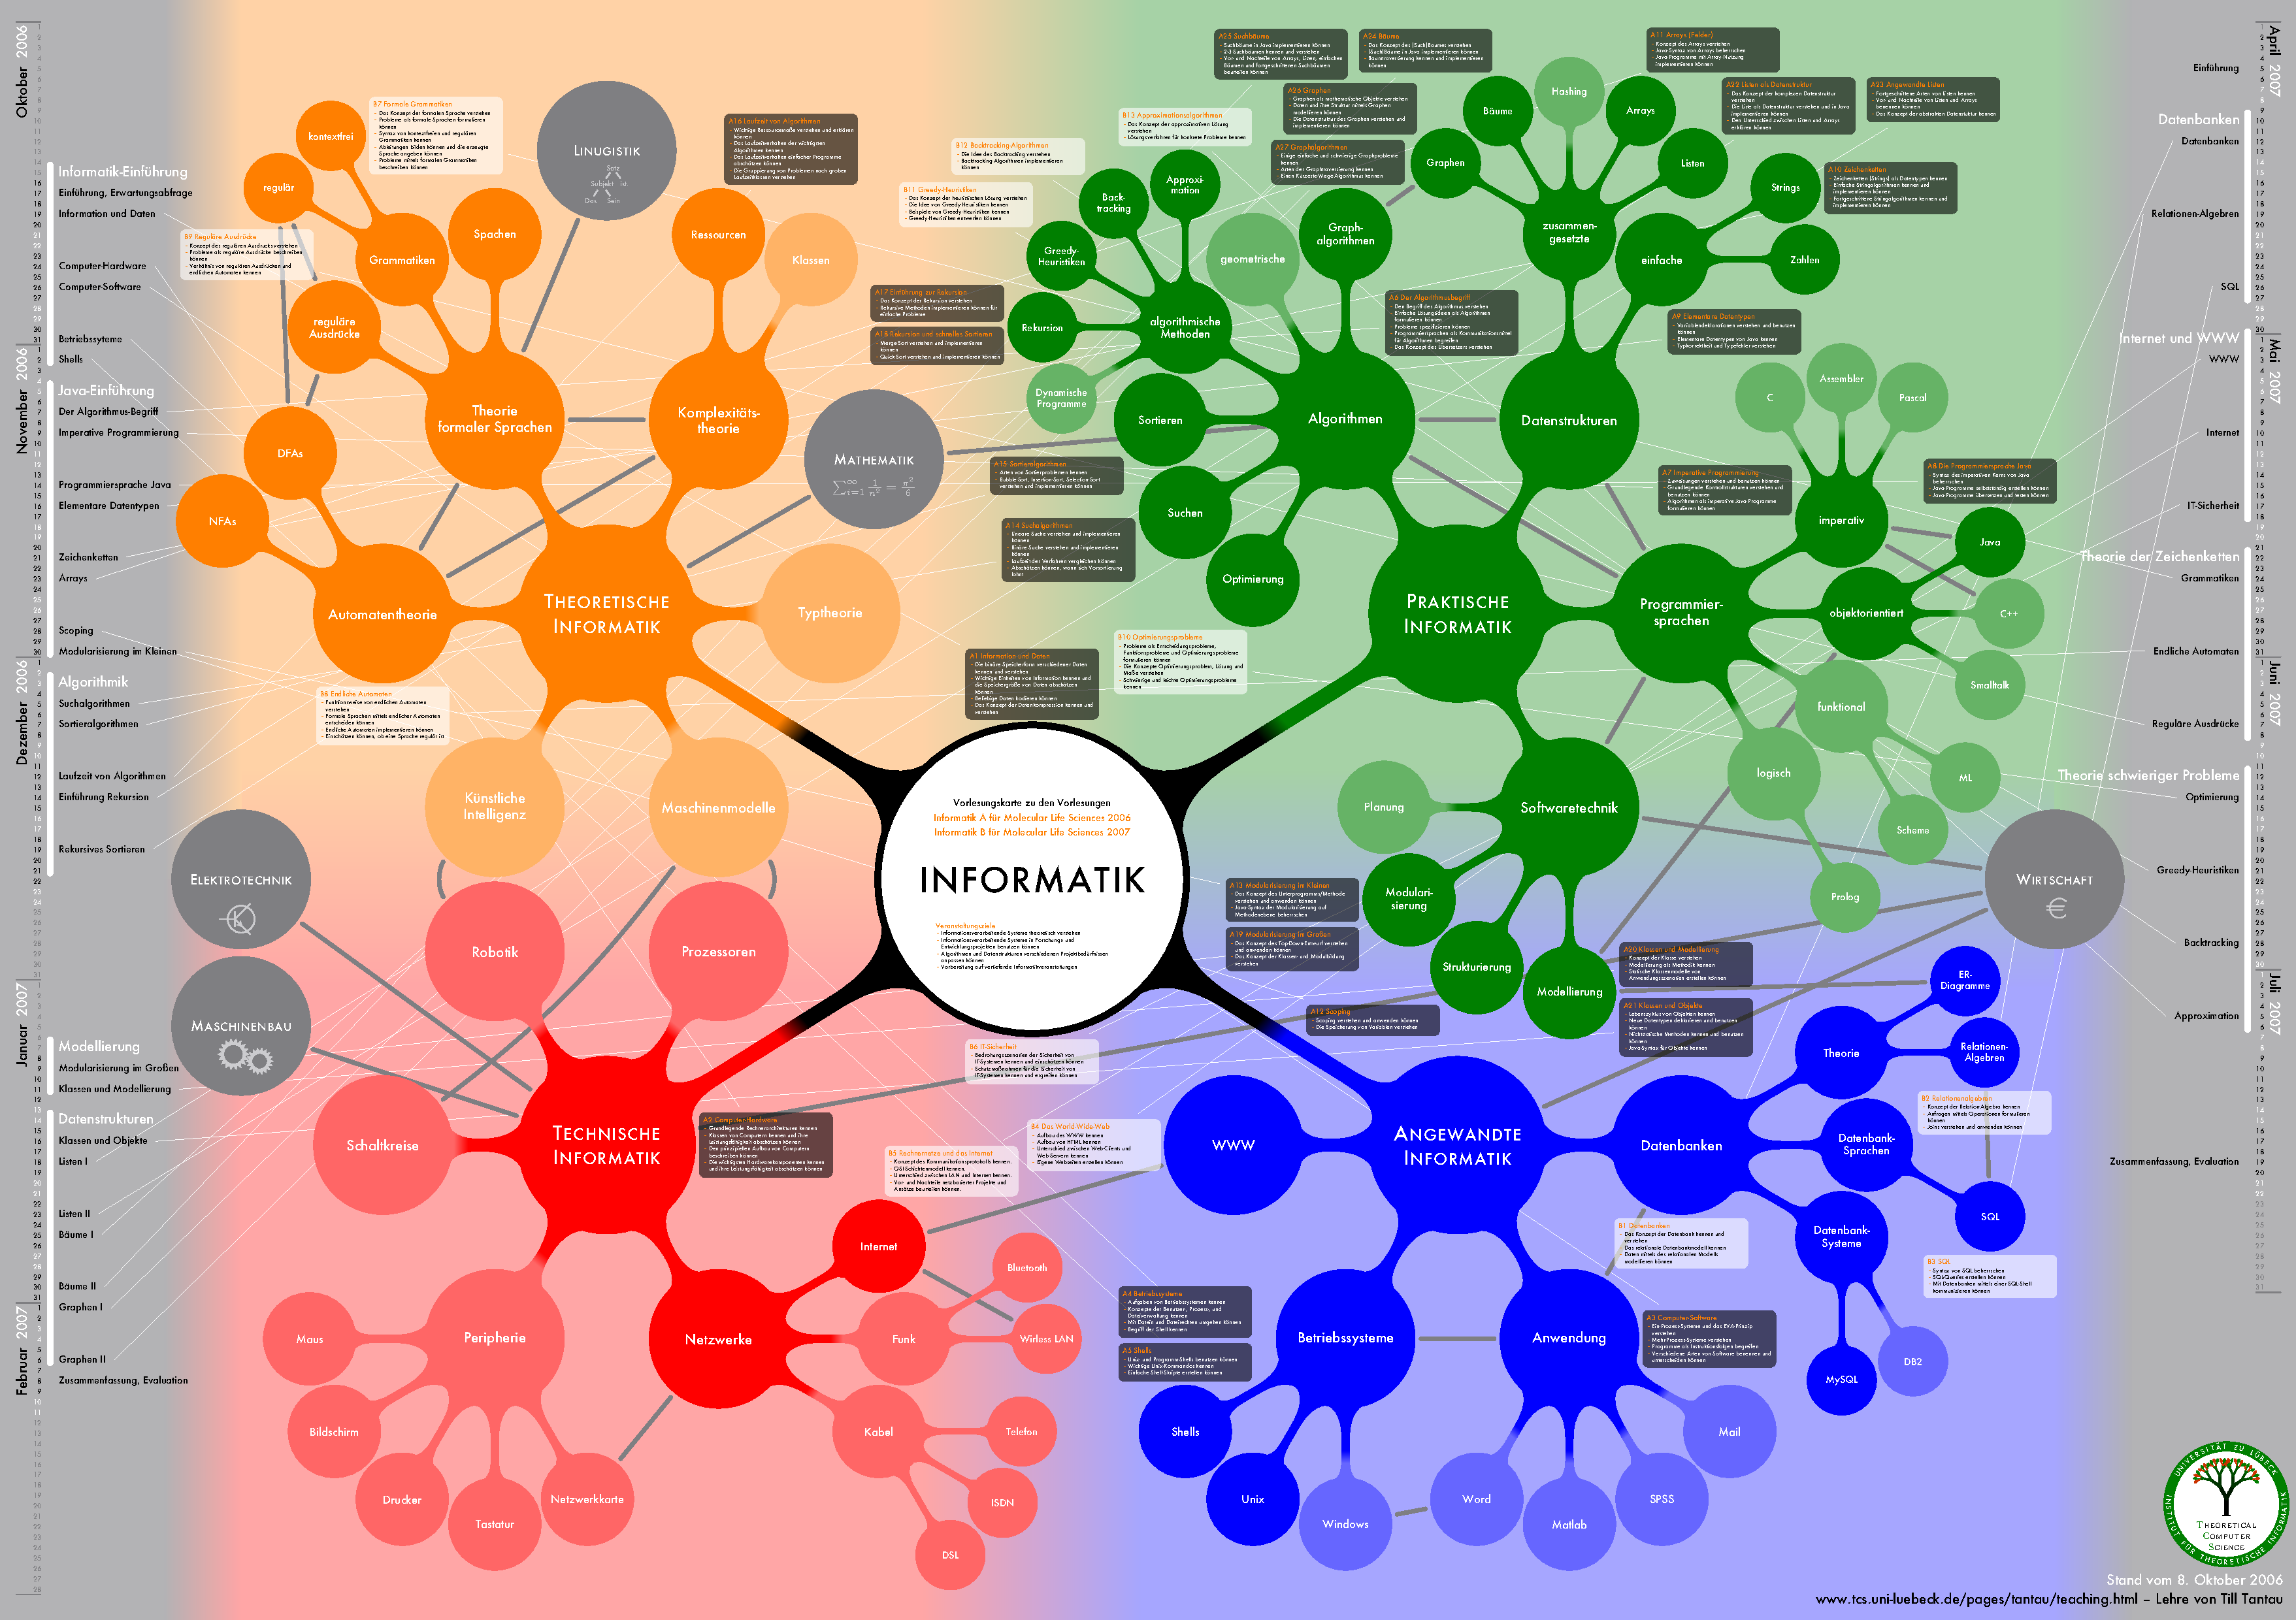
\includegraphics[width=\textwidth]{pgfmanual-mindmap-1.pdf}

\medskip
\noindent
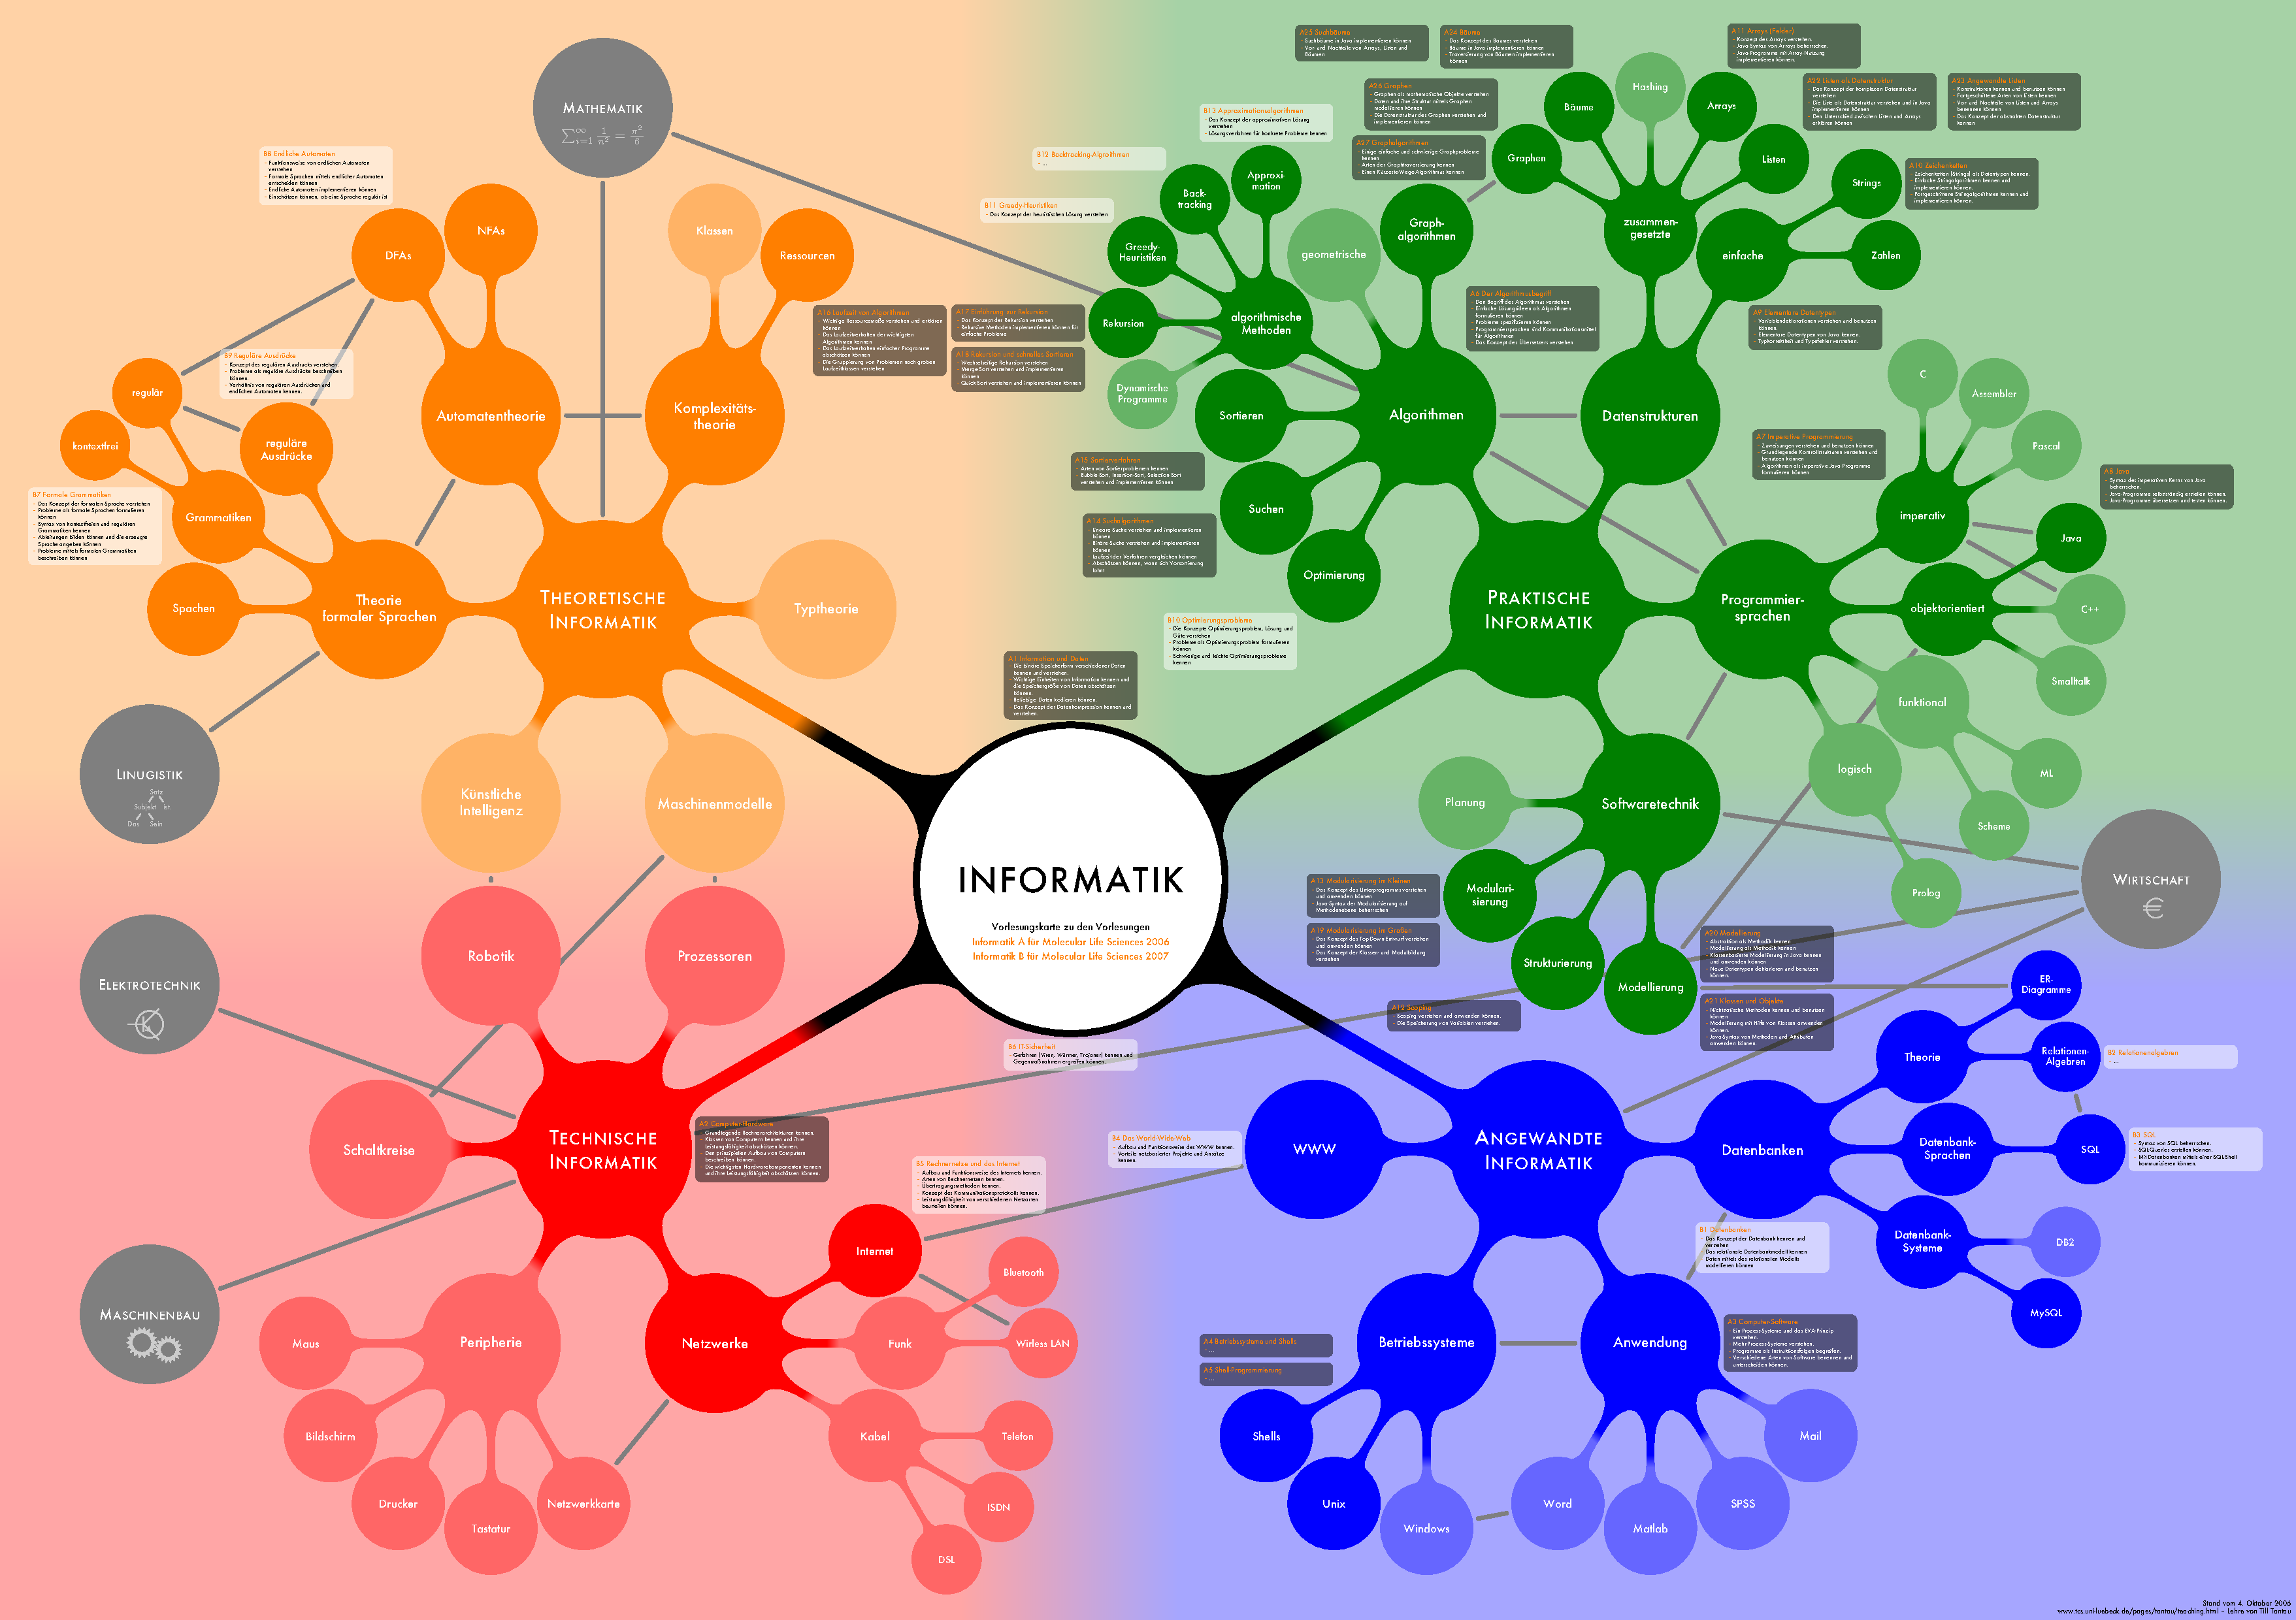
\includegraphics[width=\textwidth]{pgfmanual-mindmap-2.pdf}



%%% Local Variables: 
%%% mode: latex
%%% TeX-master: "pgfmanual-pdftex-version"
%%% End: 
